\documentclass[a4paper,11pt,openright,oneside]{report}
\usepackage[utf8]{inputenc}
\usepackage[T1]{fontenc}
\usepackage[portuguese]{babel}
\usepackage{graphicx}
\usepackage[backend=biber, style=ieee]{biblatex}
\usepackage{csquotes}
\usepackage{blindtext}
\usepackage[printonlyused]{acronym}
\usepackage{hyperref}
\usepackage{indentfirst}
\usepackage[titletoc,title]{appendix}
\usepackage{mathtools}
\usepackage{amsmath,amsthm,amsfonts,amssymb}
\usepackage{caption}
\usepackage{subcaption}
\newcommand{\RNum}[1]{\uppercase\expandafter{\romannumeral #1\relax}}

\bibliography{report.bib}

\begin{document}

\begin{titlepage}
\begin{center}

{\vspace*{50mm}\textsc{\Huge\textbf{Bloom-filter + Locality-Sensitive Hashing}\\ \small{Métodos Probabilísticos para Engenharia Informática}}}\\[2cm]
{\textsc{\small\textbf{Universidade de Aveiro}}}\\[0.5cm]
{\small Pedro Martins 76551\\Ricardo Jesus 76613}\\[0.5cm]
{\small	17 de Dezembro de 2015}\\

\begin{figure}[b]
\center
\graphicspath{}

\includegraphics[height=2cm]{ua.pdf}
\end{figure}

\end{center}

\end{titlepage}

\title{\textbf{Bloom-filter + Locality-Sensitive Hashing}\\[1cm]\textsc{\small {Departamento de Electrónica, Telecomunicações e Informática} \\ \large {UNIVERSIDADE DE AVEIRO}}}
\author{Pedro Martins 76551, pbmartins@ua.pt\\Ricardo Jesus 76613, ricardojesus@ua.pt}
\date{17 de Dezembro de 2015}

\maketitle

\pagenumbering{roman}

\begin{abstract}

ABSTRACT

\end{abstract}

\tableofcontents
%\listoftables
\listoffigures

\clearpage
\pagenumbering{arabic}

\chapter{Introdução}
\label{chap.introdução}

Na área da informática, muitas vezes é necessário saber se algo pertence a conjunto de forma eficiente. Em muitas linguagens de programação, a maneira mais comum seria percorrer todo o conjunto e comparar, um a um, todos os elementos até encontrar o que se inicialmente andava à procura. No entanto, este método é deveras ineficiente, principalmente se se estiver a trabalhar com conjuntos com milhões ou mais elementos, e aí que surgem os \textit{Bloom-filters}. 

Este filtros usam uma ou várias funções de \textit{hashing} para determinar a pertença de um elemento no \textit{set}. São muito utilizados em grandes conjuntos de dados e em diversas aplicações como o corretor ortográfico dos computadores, \textit{smartphones}, etc., análise textual, entre outras. Contudo, é um método probabilístico com um valor de erro associado.

Neste trabalho, foi desenvolvido em Matlab um \textit{Bloom-filter} e desenhada uma interface para um função de \textit{hashing} desenhada em C++ para atingir este objetivo.

\chapter{Bloom-filter}
\label{chap.bloom}

Os \textit{Bloom-filters} usam uma ou várias funções de \textit{hashing} para determinar a pertença de um elemento no \textit{set}. Deste modo, mesmo que se opere sobre um conjunto com milhões ou milhares de milhões de elementos, será sempre um processo muito mais eficiente do que se se iterasse sobre todo o \textit{set} à procura do elemento em questão (dependendo também do número e da qualidade das funções de \textit{hashing} utilizadas).

No entanto, é um método probabilístico, e tem um erro associado. Na criação de um \textit{Bloom-filter} define-se sempre um erro máximo esperado, erro esse que apenas ocorre na "inclusão", isto é, um membro que à partida já se saiba que pertença ao conjunto nunca será considerado não pertencente, mas alguns membros que, à partida, se saiba que não estão no \textit{set}, podem ser considerados como pertencentes ao conjunto.

Para diminuir esse erro, por norma, para além de aumentar o tamanho do \textit{set}, usa-se um número variado de funções de \textit{hashing} descorrelacionadas entre si, em vez de utilizar apenas uma. Isto permite que os resultados do \textit{hashing} estejam mais dispersos por todo o vetor. Neste caso, em vez de utilizarmos k funções diferentes, utilizaremos a família de funções \textit{FarmHash}, desenvolvida pela Google, em que um dos argumentos, a \texttt{seed}, especifica cada uma das funções.

Na implementação do filtro neste trabalho (\textit{BloomFilter.m}) foi desenvolvida uma classe, baseada num \textit{Counting Bloom-filter} (conta-se o número de vezes que cada elemento é adicionado ao filtro), com 5 atributos:
\begin{description}
\item[k]
Número de funções de \textit{hashing} utilizadas.
\item[byteArray]
Limite de vezes que o contador de cada posição é incrementado (255).
\item[arraySize]
Tamanho do vetor de \textit{bits}.
\item[amountAdded]
Número total de elementos adicionados ao \textit[array].
\item[expectedMaxSize]
Tamanho do conjunto que se pretende adicionar do vetor.
\end{description}

No construtor da classe, são calculados os valores do tamanho do vetor (\texttt{arraySize}) e do número de funções de \textit{hash} necessárias, consoante os valores passados como argumentos do próprio construtor, a probabilidade de falsos positivos, isto é, o erro esperado (\texttt{falsePositiveProbability}) e o tamanho do conjunto que se pretende adicionar ao vetor (\texttt{expectedMaxSize}). 

Assumindo que a probabilidade de falsos positivos $p$ é

$$ p =  \left(1 - e^{-\frac{km}{n}}\right)^k $$

e, usando o tamanho do vetor de \textit{bits} $n$ e o tamanho do conjunto que queremos adicionar ao filtro $m$,

$$ a = \left(1 - \frac{1}{n}\right)^m $$

para determinar o número $k$ ótimo de funções de \textit{hashing} que se devem utilizar, deduz-se que

$$ \ln p = k * \ln \left(1 - a^k\right) \\
\Leftrightarrow k =  \frac{n * \ln 2}{m}$$

A partir das fórmulas acima encontradas, também se deduz que

$$ n = \frac{m * \ln \left(\frac{1}{p}\right)}{\left(\ln 2\right) ^ 2} $$

Para além do construtor, existem também métodos para adicionar e verificar a existência de elementos no filtro.

\begin{description}
\item[getIndexes]
Devolve os vários índices para os quais a função de \textit{hashing} aplicada à \textit{string} passada como argumento aponta.
\item[add]
Adiciona um elemento ao filtro.
\item[contains]
Verifica se o elemento passado como argumento existe no filtro (poderá haver ocorrência de falsos positivos).
\item[count]
Devolve o número de vezes que um dado elemento foi adicionado ao vetor.
\item[remove]
Remove do filtro, caso exista, o elemento passado como argumento.
\item[maxCount]
Devolve o número máximo de vezes que um elemento foi adicionado ao vetor.
\item[minCount]
O inverso da função \texttt{maxCount}.
\item[Setters]
Coleção de funções utilizadas para modificar os atributos do \textit{Bloom-filter}, caso o campo \texttt{debug} (argumento passado ao construtor) esteja com o valor 1.
\end{description}

\section{Testes}
\label{sec.bloomtests}

Para testar este módulo, foram desenvolvidos diversos, de entre os quais uns para verificar qual seria o número ideal de funções de \textit{hashing} (\texttt{k}) e outro para verificar o tamanho ideal do vetor de \textit{bits} (\texttt{n}).

No entanto, também foram realizados outros testes relativamente às funções de \textit{hashing} utilizadas pelo \textit{Bloom-filter}.

\subsection{Distribuição de funções de \textit{hashing}}
\label{subsec.hashdist}

Este módulo (\textit{test\_hashFunction\_distribution.m}) tem como principalmente objetivo provar que as funções de \textit{hashing} têm uma distribuição uniforme, para diversos valores de \texttt{k} (neste caso, irá variar entre 1 e 10).

A família de funções de \textit{hashing} usada tanto no filtro como nos testes é designada por \textit{FarmHash}, desenvolvida pela Google. Foi apenas criada uma interface para que pudesse ser usada em Matlab.

Neste teste, foi gerado um conjunto de \textit{strings} aleatórias, usando a função \texttt{generateStrings}, que aceita como argumentos o tamanho do conjunto que devolverá e o tamanho máximo das \textit{strings} que irá gerar (caso o terceiro argumento seja 0, elas terão tamanho fixo, caso contrário, será definido como tamanho máximo), e gerados diversos valores de \textit{hashing}, consoante os diversos elementos do conjunto e da \texttt{seed} correspondente.

As distribuições para cada valor de \texttt{k} deverão ser o mais uniformes possíveis, e os resultados comprovam-no, tal como se pode ver nos histogramas da \autoref{fig:hashdist}.

\begin{figure}[ht]	
\center
\fbox{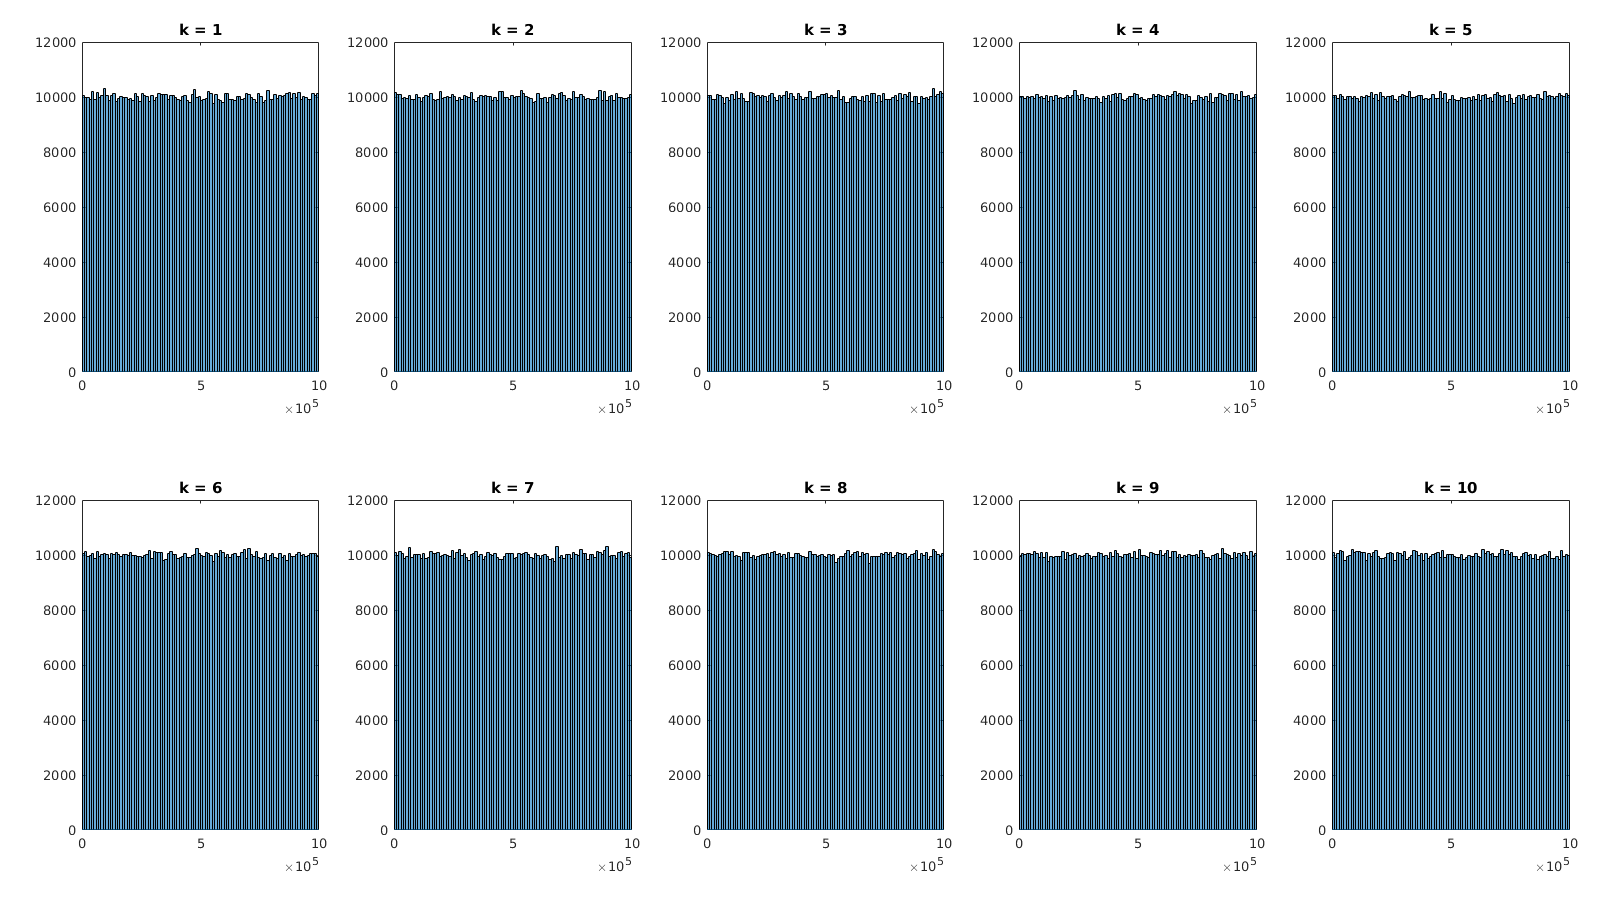
\includegraphics[height=5cm]{img/test_HashFunction_distribution}}
\caption{Resultados das distribuições das \texttt{k} funções de \textit{hashing}}
\label{fig:hashdist}
\end{figure}

\subsection{Correlação das funções de \textit{hashing}}
\label{subsec.hashcorr}

Para que se possam ser utilizar as várias funções de \textit{hashing}, é necessário que as mesmas sejam descorrelacionadas, isto é, que o coeficiente de correlação seja 0. No entanto, neste caso, considerar-se-á um erro de 0.01 (é quase impossível que os valores sejam iguais a zero, portanto, aceita-se esta ligeira variação).

Este módulo encontra-se no ficheiro \textit{test\_hashFunction\_correlation.m} e, tal como noutros testes, gerar-se-á um \textit{set} de \textit{strings} aleatórias e os respetivos valores de \textit{hashing} para diferentes valores de \texttt{k}, a variar entre 1 e 10. Foi também criada uma matriz de dimensões \texttt{k} por \texttt{numTests}, isto é, cada linha terá diferentes valores de \textit{hashing} para um mesmo valor de \texttt{k}. De seguida, calcular-se-ão os coeficientes de correlação entre de cada conjunto de \textit{hash codes} (linha) desses mesmos valores com o auxílio da função \texttt{corrcoef} (calcula o coeficiente de correlação entre dois conjuntos, neste caso, duas linhas distintas).

Por fim, é gerado um gráfico recorrendo à função \texttt{surf} para mostrar os valores de correlação resultantes. Como verificamos, todos os valores situam-se abaixo do erro assumido (à exceção dos valores em que assumimos o mesmo valor de \texttt{k}, isto é, compararmos a mesma linha, sendo que, nesse caso, o valor será 1), daí se poder considerar que as funções de \texttt{hashing} são descorrelacionadas, tal como se pretendia.

\begin{figure}[ht]	
\center
\fbox{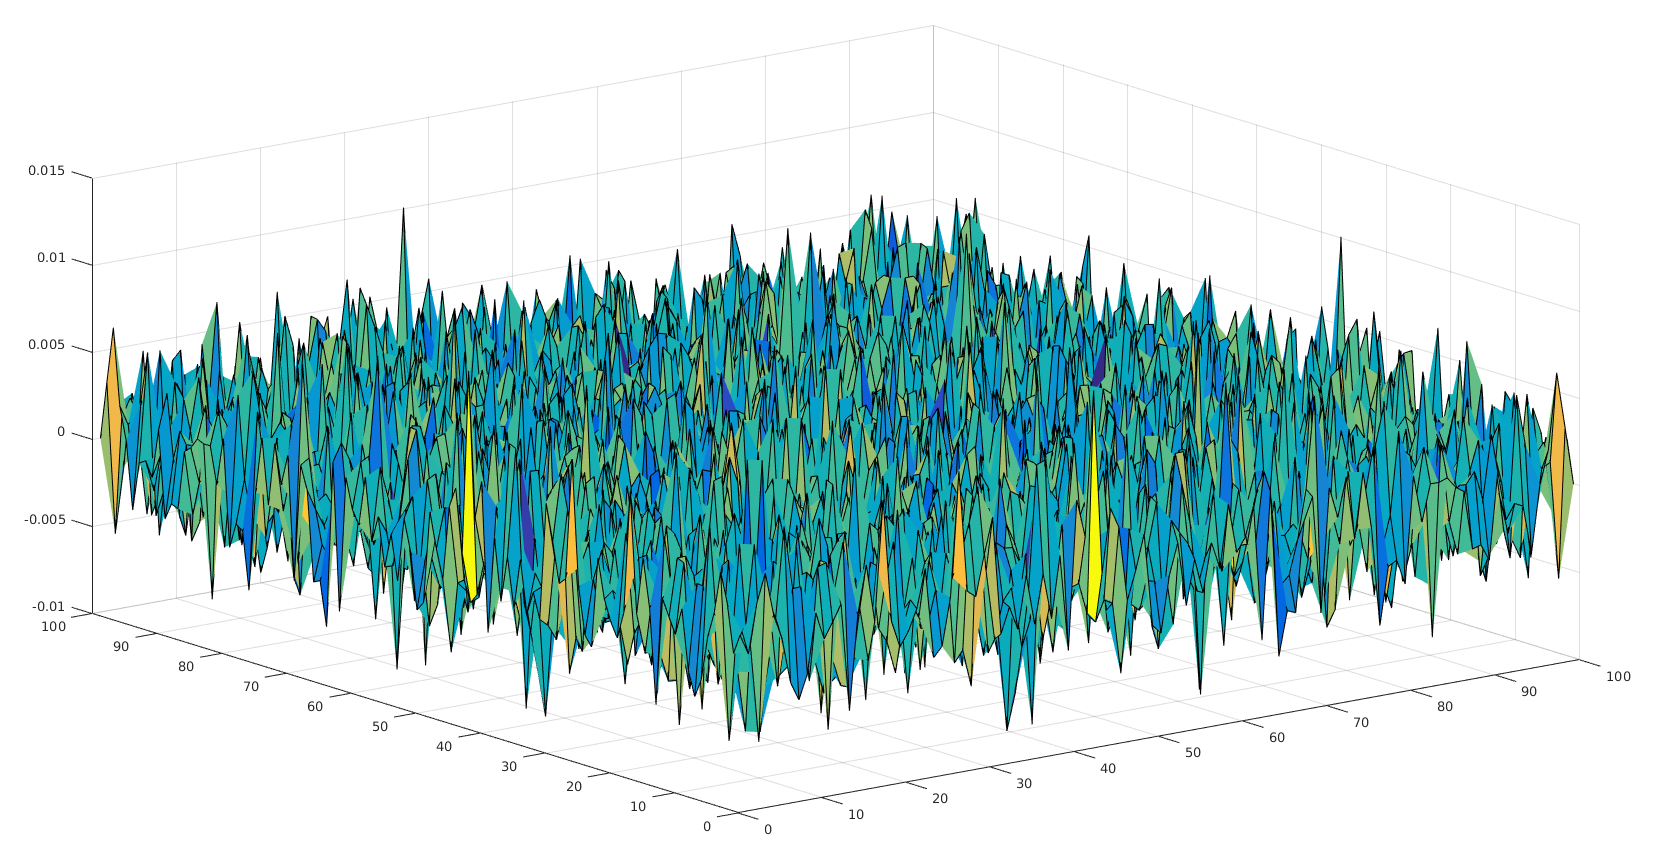
\includegraphics[height=5cm]{img/test_HashFunction_decorrelation}}
\caption{Resultados do teste de correlação de \texttt{k} funções de \textit{hashing}}
\label{fig:hashcorr}
\end{figure}

\subsection{Independência das funções de \textit{hashing}}
\label{subsec.hashindep}

Para além do teste de correlação, foi também efetuado um teste de independência das funções de \textit{hashing} (\textit{test\_hashFunction\_independence.m}), adaptado da implementação do professor António Teixeira. A independência implica descorrelação, e com isto, pode-se provar com qualquer um dos testes que as funções são descorrelacionadas. O objetivo é provar que cada par de colunas é independente entre si.

Primeiramente, é criado um \textit{set} de cem mil \textit{strings} aleatórias e, seguidamente, outra matriz dos respetivos \textit{hash codes} com \texttt{k} (neste teste, \texttt{k = 10}) diferentes \textit{seeds}, utilizando a família de funções \textit{FarmHash}, de tamanho \texttt{k} (número de funções de \textit{hashing} que se pretende aplicar) por \texttt{N} (número de testes que se pretendem executar). De seguida, é gerado um vetor de 10 elementos linearmente espaçados (\texttt{x}) entre 0 e \texttt{N}, e, para cada par de colunas, é criada uma matriz (\texttt{pmf}) de dimensão \texttt{length(x) - 1 / length(x) - 1}. Depois, guarda-se em cada elemento da matriz o número de elementos das colunas de \textit{hash codes} que se situam num mesmo intervalo (esse intervalo é definido pelo vetor \texttt{x} já criado).

Por fim, é calculada a matriz de probabilidade conjunta de duas colunas (\textit{PMF - Probability Mass Function}), e, a partir da mesma, são calculados os vetores de probabilidade individuais de cada uma das colunas. Finalmente, é calculado o resultado da multiplicação destes dois últimos vetores (dois acontecimentos A e B são independentes se $P(A\&B) = P(A) * P(B)$), e compara-se com a matriz de probabilidade conjunta.

\begin{figure}[ht]	
\center
\fbox{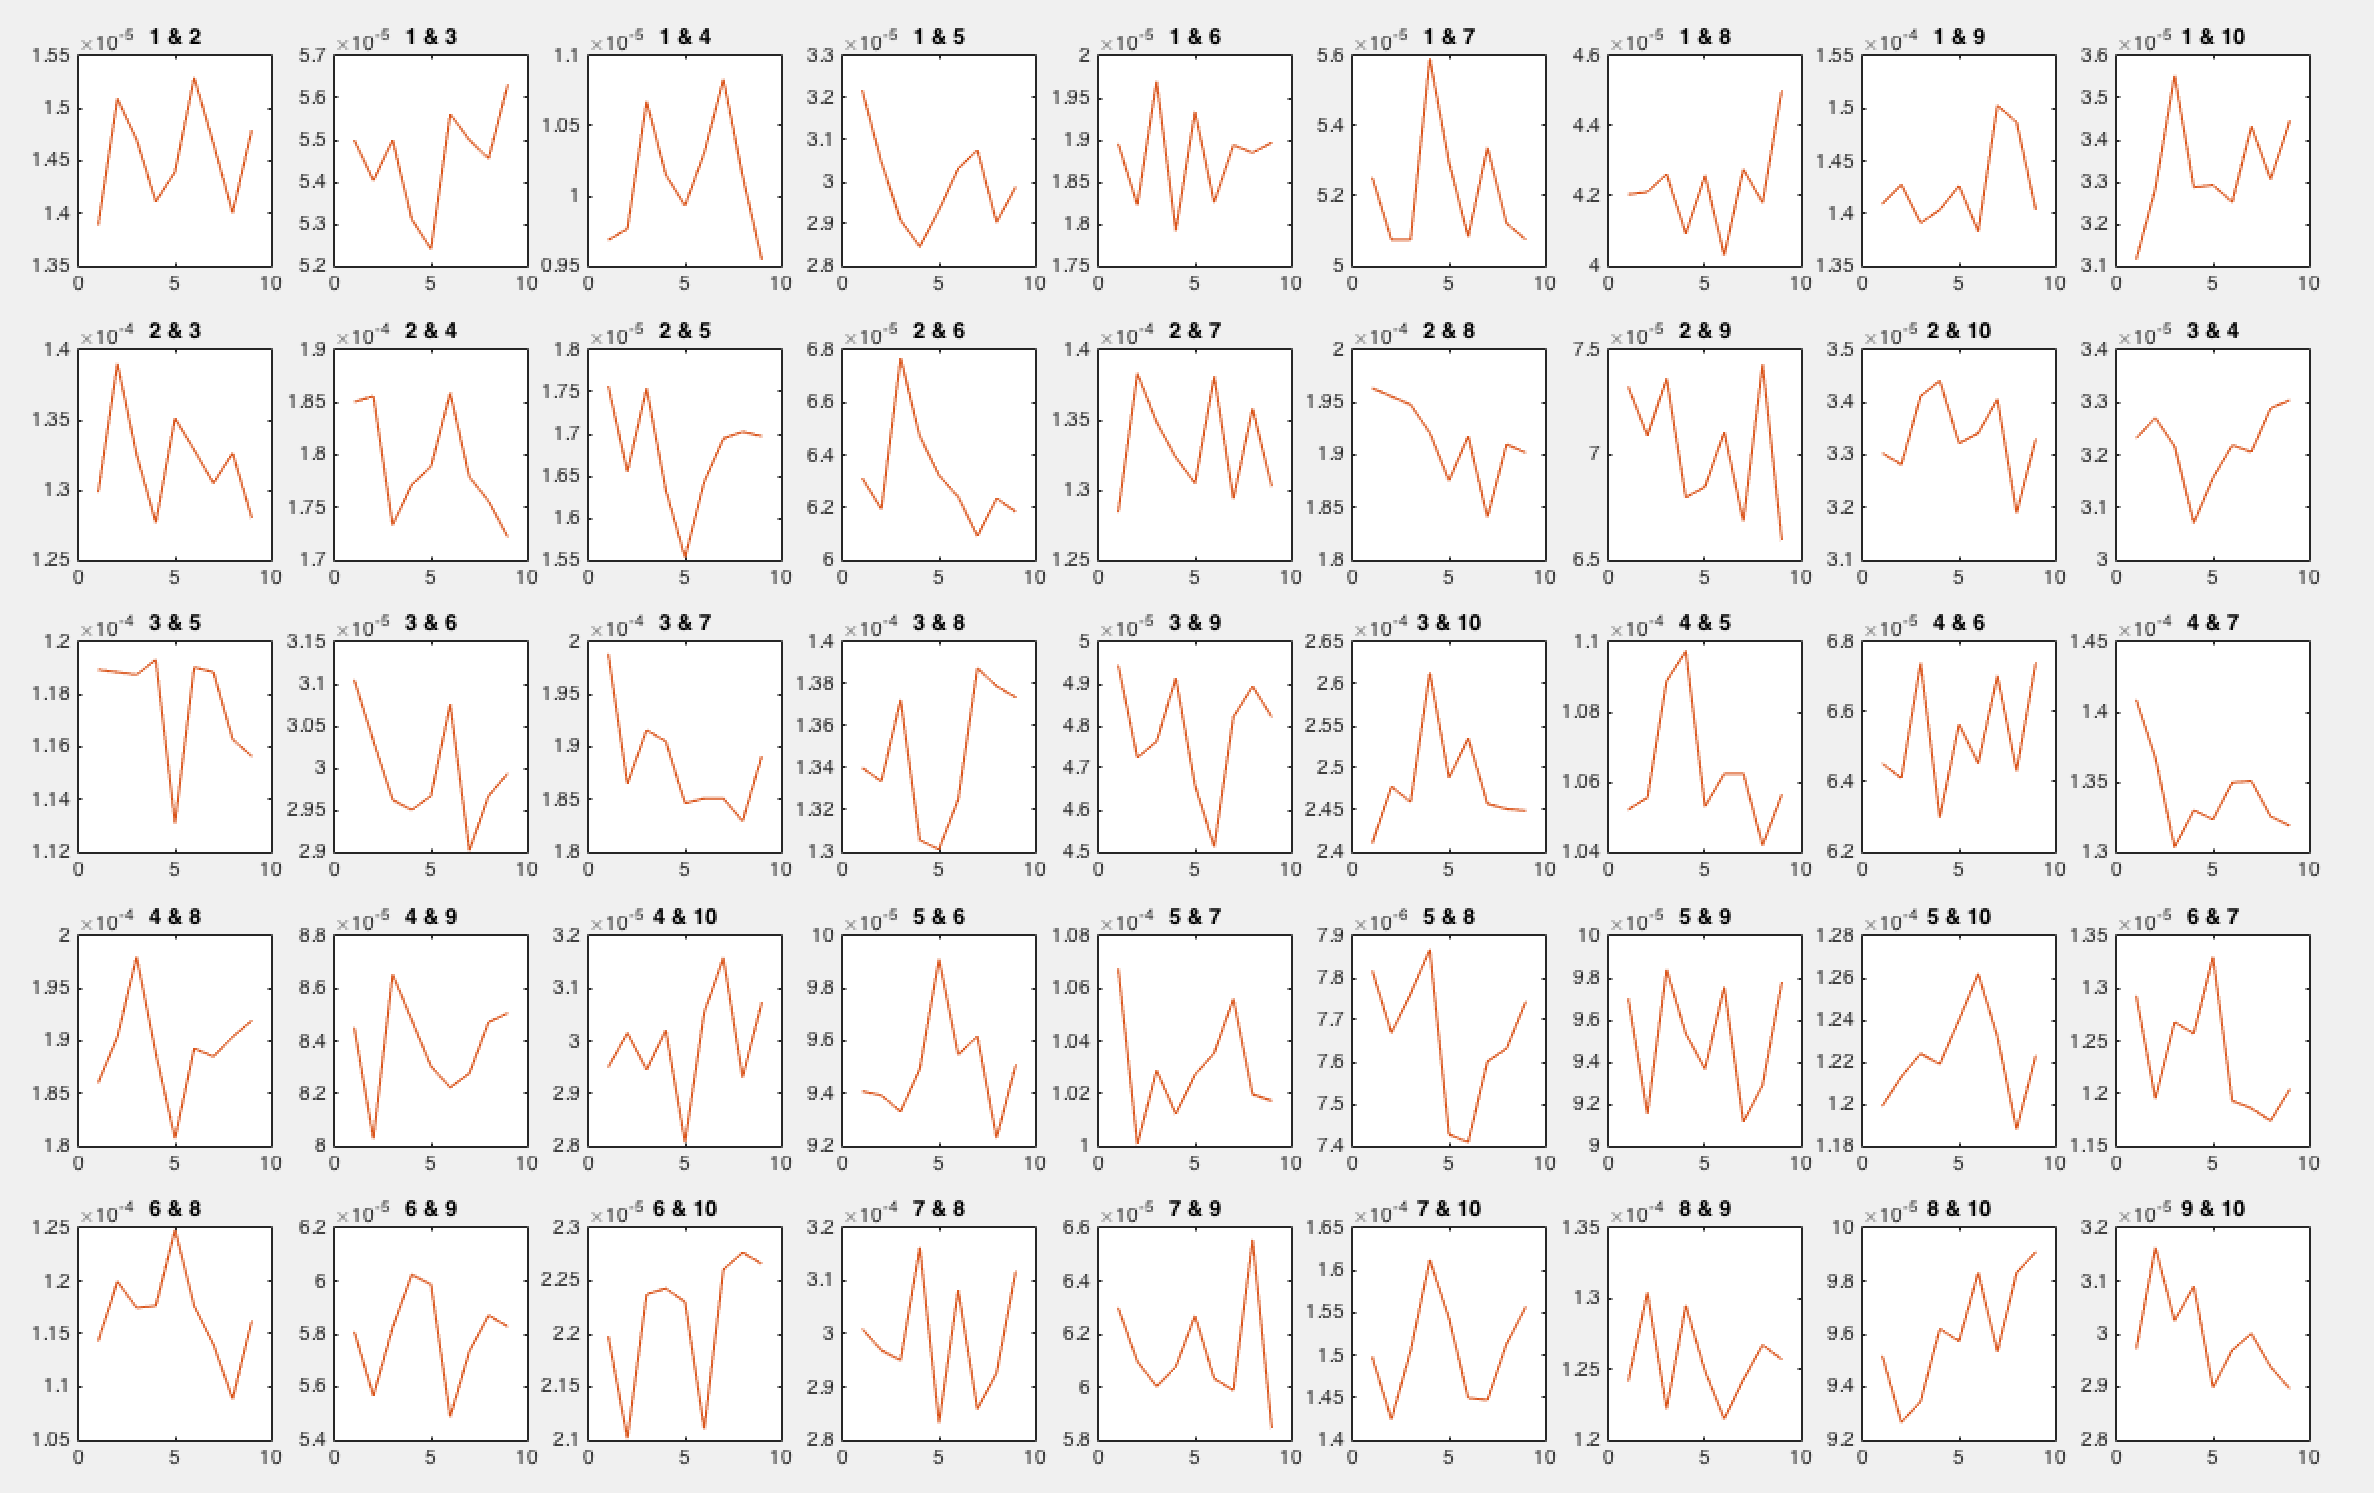
\includegraphics[height=7cm]{img/test_hashFunction_independence}}
\caption{Resultados do teste de independência de \texttt{k} funções de \textit{hashing}}
\label{fig:hashindep}
\end{figure}

Como os valores da variação de resultados são mínimos (como se observa na \autoref{fig:hashindep} todos os valores rondam os $10^-4$), podemos considerar que a família de funções é independente, o que nos leva a concluir que são descorrelacionadas.

\subsection{Número ideal de funções de \textit{hashing}}
\label{subsec.optimalk}

O programa de teste para o valor de \texttt{k} ideal encontra-se com o nome \textit{test\_optimalK.m}.

Começa-se por criar uma instância da classe de \textit{Bloom-filter} anteriormente desenvolvida (com o campo \texttt{debug} inicializado a 1, para que se possam utilizar as funções de alteração de valores) e gerar dois conjuntos (um dos quais será adicionado ao filtro, outro não) distintos de cem mil (valor que pode ser alterado) \textit{strings} (como poderá haver \textit{strings} iguais nos \textit{sets}, o tamanho será sempre ligeiramente inferior ao definido anteriormente). De seguida, define-se o tamanho do vetor de \textit{bits} do filtro como oito vezes maior do que o tamanho dos conjuntos de \textit{strings} gerados.

Por fim, itera-se sobre um vetor de \texttt{k} que se definira anteriormente (neste caso, é um vetor com valores de 1 a 15) e, cada ciclo, define-se um \texttt{k} no \textit{Bloom-filter}, adiciona-se os elementos do vetor incialmente escolhido como aquele que se iria adicionar ao filtro e verifica-se se algum dos elementos do outro conjunto de \textit{strings} pertence ou não ao filtro. Caso pertença, é incrementado um contador, para, no final do ciclo, ser calculada a probabilidade de falsos positivos.

\begin{figure}[ht]	
\center
\fbox{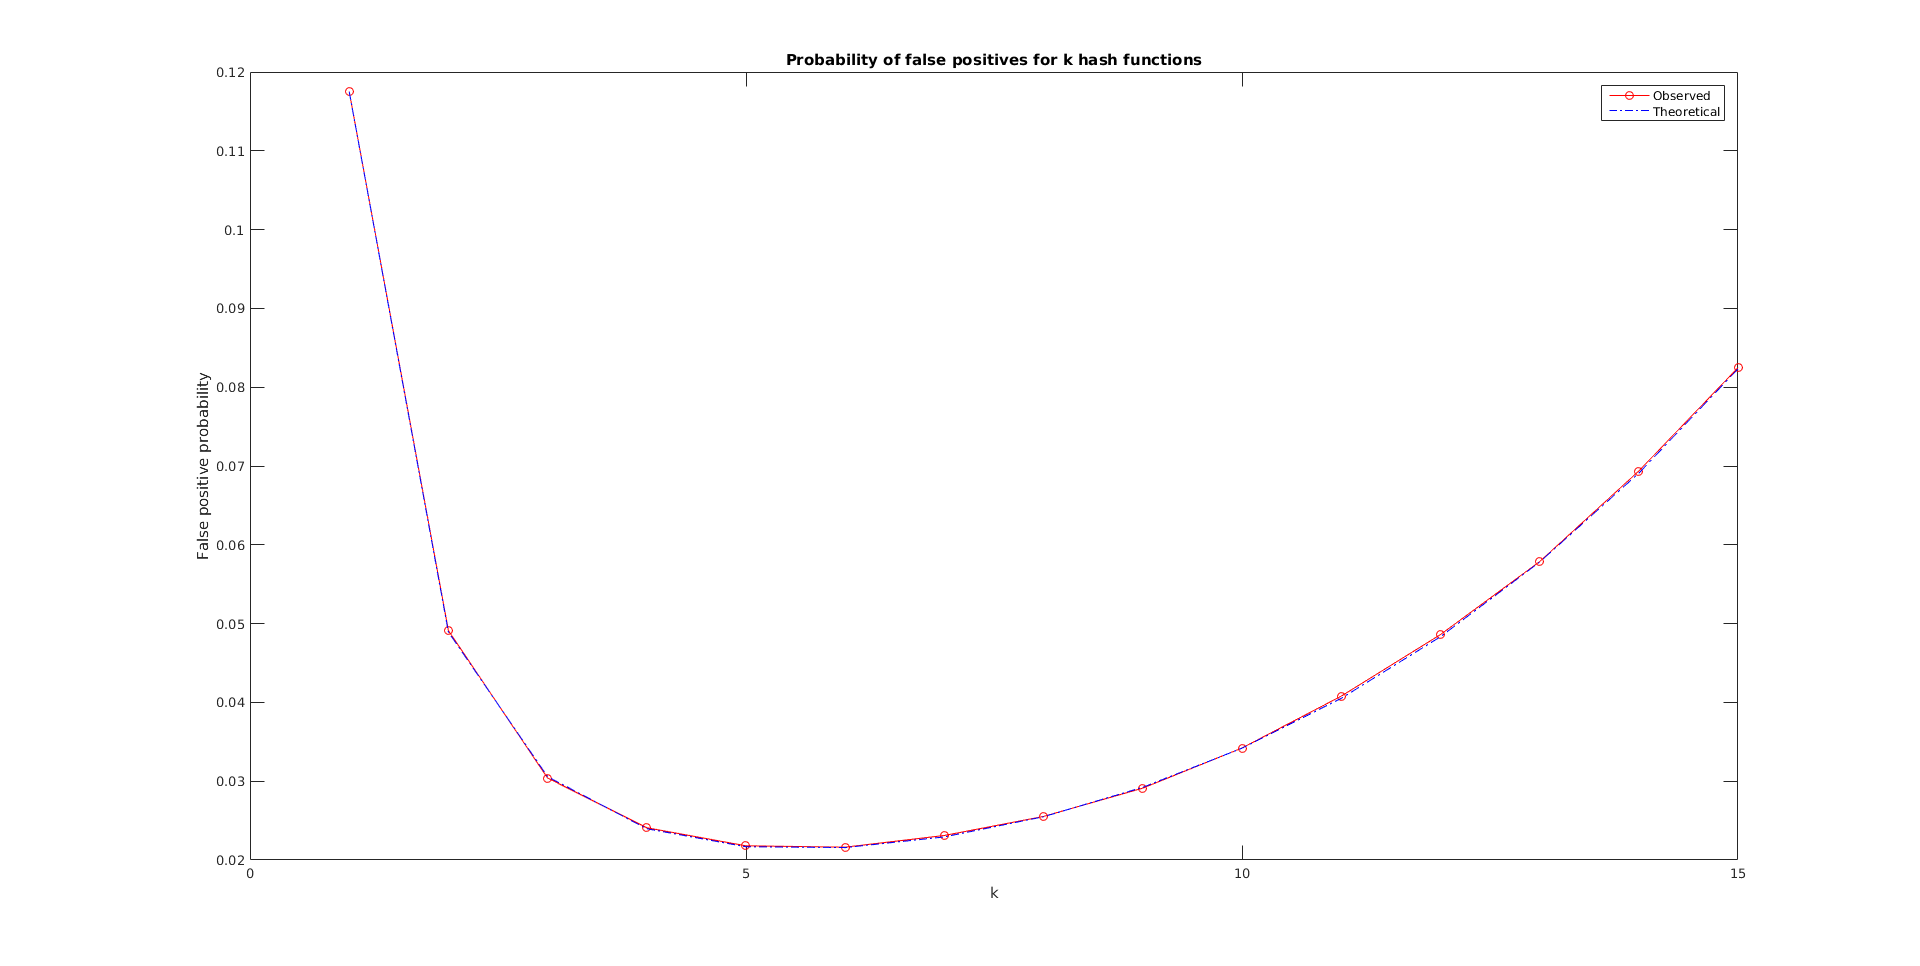
\includegraphics[height=5cm]{img/test_OptimalK}}
\caption{Resultados do teste do valor ideal de funções de \textit{hashing} (\texttt{k})}
\label{fig:optimalk}
\end{figure}

De acordo com o gráfico da \autoref{fig:optimalk}, usando a fórmula 

$$ p =  \left(1 - e^{-\frac{km}{n}}\right)^k $$

para determinar a probabilidade de falsos positivos (teórica) para diferentes valores de \texttt{k} e usando os valores do teste acima, verificamos que as diferenças entre o valor teórico e observado são mínimas (o que significa que a função de \textit{hashing} devolve excelentes resultados, mas isso será abordado mais abaixo), e que o valor ideal é 6, para a função de \textit{hashing} em questão. Para uma função diferente, os valores poderão diferir.

\subsection{Número ideal do vetor de \textit{bits}}
\label{subsec.optimaln}

O módulo para o teste do valor ideal do tamanho do vetor \texttt{n} encontra-se no ficheiro \textit{test\_optimalN.m}.

Tal como no teste do \autoref{subsec.optimalk}, também são criados dois conjuntos de \texttt{strings} aleatórias com o mesmo propósito, um para ser adicionado ao filtro e o outro não. É também criado um vetor com diferentes valores de \texttt{n}, que vão desde o tamanho dos conjuntos de \textit{strings} até 10 vezes esse valor, com uma diferença de metade do mesmo valor entre cada.

De seguida, itera-se sobre os valores deste último vetor de valores e vai-se criando uma instância de um \textit{Bloom-filter} com os valores de \texttt{n} (\texttt{arraySize}) e \texttt{k} (depende do tamanho do vetor) a cada passagem. Adiciona-se um dos conjuntos de \textit{strings}, verifica-se a existência dos elementos do outro que não foi adicionado e, por fim, calcula-se a probabilidade de falsos positivos, tal como no teste anterior.

\begin{figure}[ht]	
\center
\fbox{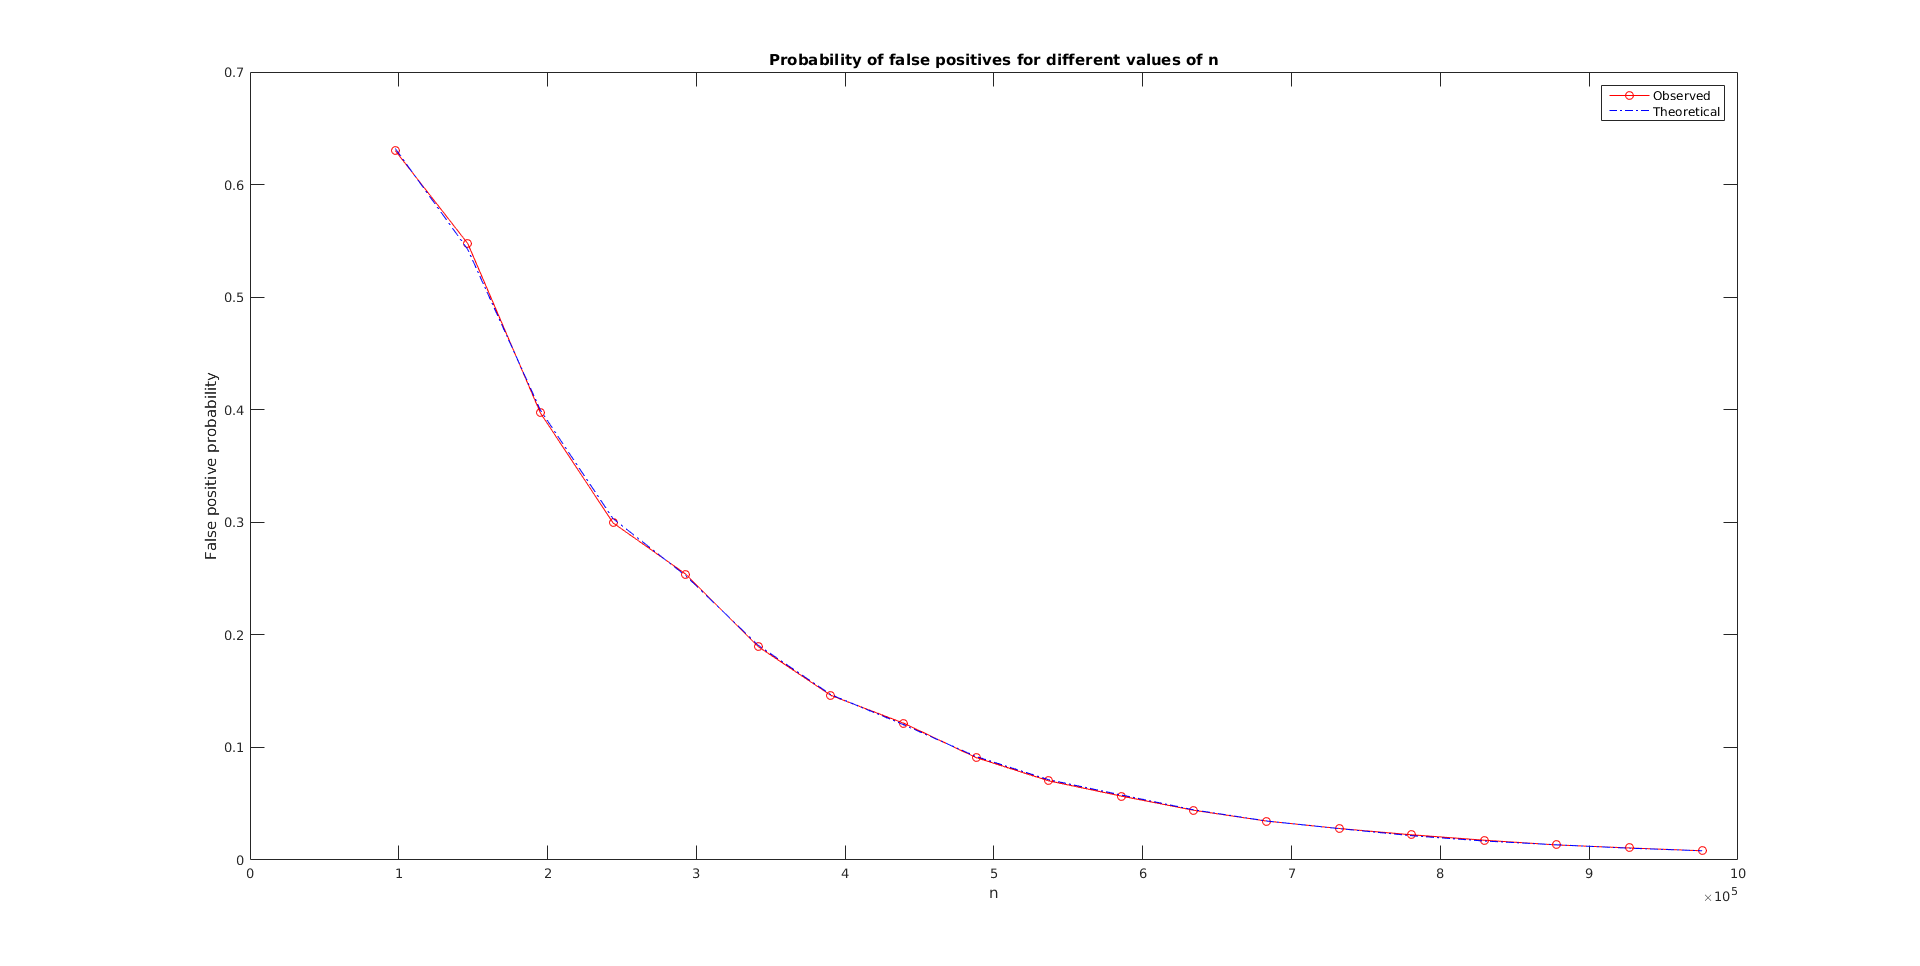
\includegraphics[height=5cm]{img/test_OptimalN_img}}
\caption{Resultados o teste do tamanho ideal do vetor de \textit{bits} (\texttt{arraySize} / \texttt{n})}
\label{fig:optimalnimg}
\end{figure}

Como se verifica no gráfico da \autoref{fig:optimalnimg}, à medida que o tamanho do \textit{array} aumenta, a probabilidade de falsos positivos diminui, isto é, são inversamente proporcionais.

Os valores ideias são os presentes na \autoref{fig:optimalntext}

\begin{figure}[ht]	
\center
\fbox{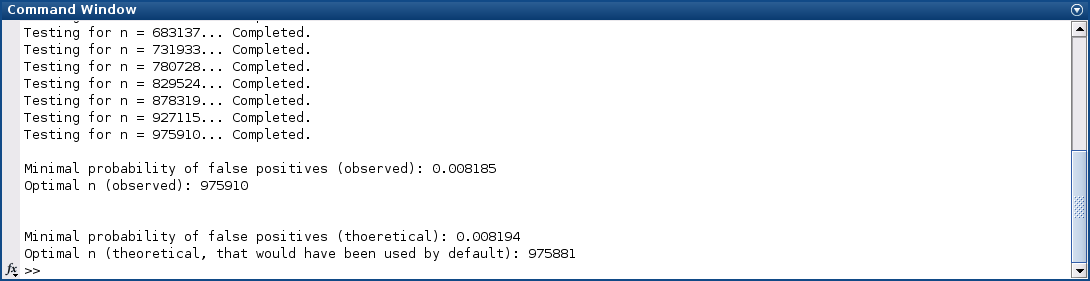
\includegraphics[height=5cm]{img/test_OptimalN_txt}}
\caption{Resultados ideias do tamanho ideal do vetor de \textit{bits} (\texttt{arraySize} / \texttt{n})}
\label{fig:optimalntext}
\end{figure}

\subsection{Testes práticos do \textit{Bloom-filter}}
\label{subsec.testebloom}

Foram desenvolvidos dois módulos semelhantes para um teste mais direcionado ao uso real de um \textit{Bloom-filter}. Estão em dois ficheiros distintos, \textit{test\_big\_BloomFilter.m} e \textit{test\_small\_BloomFilter.m}.

O primeiro segue o modelo dos testes anteriores, em que se gera dois \textit{sets} de um certo tamanho (neste caso, cem mil elementos) de \textit{strings} aleatórias, cria-se uma instância de um \textit{Bloom-filter} com uma probabilidade de falsos positivos de 0.0001\%, adiciona-se um dos conjuntos ao filtro e verifica-se a existência de falsos positivos. Por fim, compara-se o resultado observado da probabilidade de falsos positivos com a que se definiu aquando a criação do filtro. O objetivo é que os resultados sejam o mais próximos possíveis, algo que se conseguiu atingir em ambos os testes.

No segundo teste (\textit{small}), contrariamente ao primeiro em que se geram os conjuntos, definem-se conjuntos muito pequenos inicialmente e, depois, executa-se o mesmo processo que o anterior.

\begin{figure}[ht]	
\center
\fbox{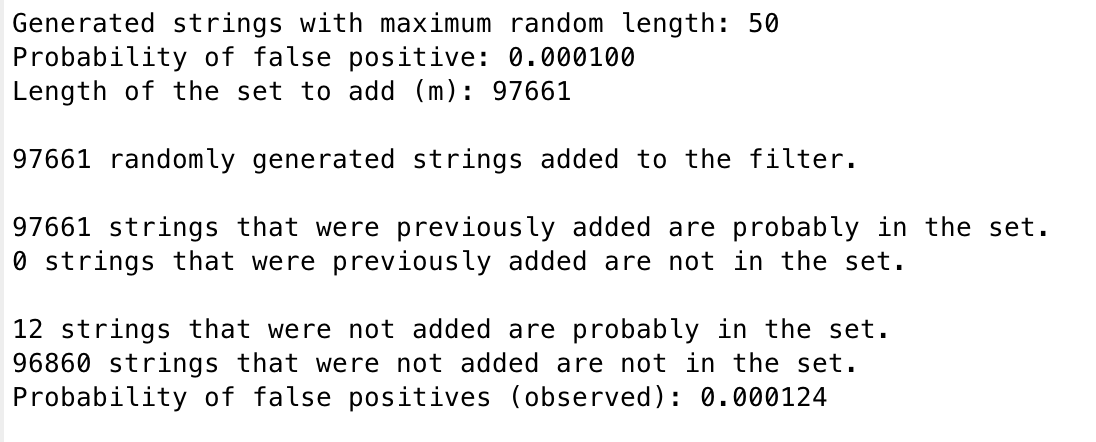
\includegraphics[height=5cm]{img/test_big_BloomFilter}}
\caption{Resultados da execução de \textit{test\_big\_BloomFilter.m}}
\label{fig:testbigbloom}
\end{figure}


\section{Locality-Sensitive Hashing}
\label{sec.lsh}

O \textit{Locality-Sensitive Hashing} é particularmente útil quando se têm grandes conjuntos de documentos e se pretendem achar semelhantes entre si, como, por exemplo, achar notícias semelhantes em diversos \textit{websites}. No entanto, pequenos trechos dos documentos podem aparecer noutros não necessarimente na mesma ordem. Para além do mais, se tivermos \textit{sets} na ordem dos milhões e milhares de milhão, são tantas comparações que são necessárias fazer que excedem a memória disponível.

Portanto, para podermos comparar documentos, são necessários 3 passos:

\begin{description}
\item[Shingling]
Converter documentos para conjuntos.
\item[Min-Hashing]
Converter grandes conjuntos para pequenas assinaturas (por norma, de inteiros), preservando a similariedade.
\item[Locality-Sensitive Hashing]
Forcar-se apenas nos pares de assinaturas que possivelmente pertençam a documentos semelhantes, e mais tarde testar realmente a sua similariedade.
\end{description}

O módulo de \textit{LSH} está no ficheiro \textit{LSH.m} e cada função será explicada consoante o processo de exposto anteriormente.

O único construtor do módulo aceita apenas um argumento, que é o erro esperado (\texttt{expectedError}). Este erro será utilizado para calcular o número \texttt{k} de \textit{hash functions} necessárias, que é também o único atributo que o módulo possui, segundo a fórmula:

$$ k = 1 / expectedError^2 $$

\subsection{Shingling}
\label{subsec.shingling}

Uma \textit{k-shingle} de um documento é uma sequência de k \textit{tokens} (palavras, caracteres, etc.) que aparecem no documento. Documentos que tenham muitas \textit{shingles} em comum, possuem texto parecido, mesmo que o mesmo não apareça na mesma ordem.

A similariedade entre dois documentos ($D1, D2$) pode ser calculada através da Similariedade de Jaccard:

$$ sim(D1, D2) = \frac{|C1\cap C2|}{|C1\cup C2|} $$

sendo $C1$ e $C2$ os conjuntos de \textit{singles} de $D1$ e $D2$, respetivamente.

A Distância de Jaccard, por outro lado, pode ser dada por:

$$ d(D1, D2) = 1 - sim(D1, D2) $$

Para gerar um \textit{set} de \textit{singles} é utilizada a função \texttt{singleWords}, que recebe como argumento um \textit{cell array}, neste caso, de \textit{strings} (considere-se o mesmo \texttt{Doc}). Para gerar esse conjunto, é necessário selecionar quais as sequências de palavras mais importantes de \texttt{Doc}. Para tal, é necessária que seja criado um \textit{set} de \textit{stop words}, logo, foram guardadas num \textit{cell array} \texttt{stop_words} as cem palavras mais comuns da língua inglesa. Quando o programa encontra uma \textit{stop word}, ele guarda a sequência \textit{stop\_word next\_word1 next\_word2} num outro \textit{cell array}, que será o retorno da função.

\subsection{Min-Hashing}
\label{subsec.minhash}

Para contornar as demoras que as comparações de excertos de textos provocariam, os \textit{shingles} são convertidos em assinaturas de inteiros, no entanto, a similariedade tem de ser conservada.

%Neste caso, a similariedade é dada \textit{bit} a \textit{bit}, isto é, utilizando \textit{bitwise AND} como interseção e \textit{bitwise OR} como união.
Para tal, apenas se cria um vetor em que o seu valor inicial é o valor máximo de \textit{double} (auxilia no cálculo dos valores mínimos). Seguidamente, para cada valor de \texttt{k} (calculado no construtor do módulo), é gerado um vetor de assinaturas, dos quais é extraído o valor mínimo e guardado no \textit{array} previamente criado.

\iffalse





\section{Interface Web}
\label{sec.web}

Este módulo é o responsável por todas as interações entre o cliente e a aplicação. As interfaces Web comunicam com o utilizador e que, a partir das mesmas, consoante o pretendido, enviam pedidos ao servidor (de informações ou criação de ficheiros, por exemplo).

Criaram-se duas interfaces, uma aplicação para versão \textit{desktop} e outra para versão \textit{mobile}, estando elas disponíveis em \url{http://0.0.0.0:4506/web/} e \url{http://0.0.0.0:4506/mobile/}, respetivamente.

A versão \textit{desktop} é construída em \verb|HTML|, \verb|CSS| e \verb|JS|, tal como qualquer outra página Web, e tem como base o \textit{template} Greyscale, desenvolvido pela Start Bootstrap, que foi construído utilizando a \textit{framework} Twitter Bootstrap.

Por outro lado, mas utilizando as mesmas linguagens, está a aplicação para dispositivos móveis, na qual será utilizado um tema disponibilizado e baseado na \textit{framework} Ratchet.

Criaram-se várias páginas de forma a dar resposta às diversas funcionalidades disponíveis pela aplicação:

\begin{description}
\item[Index]
A página principal, onde é apresentado o projeto e os seus autores, assim como hiperligações para versão móvel e para as diversas funcionalidades da versão \textit{desktop}
\item[Página da listagem de músicas]
Página onde são listadas todas as músicas presentes na base de dados e os seus respetivos gráficos relativos a representação das notas, assim como as suas interpretações. Relativamente ás interpretações é possível o utilizador dar \textit{Like} ou \textit{Dislike} e ver quantos "gostos" e não gostos tem cada interpretação. Outra opção que tem é ouvir ou fazer download da interpretação selecionada. Para além disso, é possível ser redirecionado para a página de criar interpretações da música escolhida previamente na página que lista as músicas. 
\item[Página de criação de uma música]
Página onde é possível a criação de uma música, fornecendo um nome e a pauta no formato RTTTL.
\item[Página de criação de uma interpretação]
Acessível a partir da página da listagem de músicas carregando em \textit{create interpretation} da respetiva música que se quer criar a interpretação, é a página onde será possível a criação de uma interpretação de uma certa música, aplicando-lhe um registo e efeitos disponíveis pela aplicação
\end{description}

A comunicação com o servidor é toda ela através de JavaScript e jQuery.

A página da listagem de músicas foi construída utilizando uma função que faz uso do \texttt{\$.get()}, função de jQuery, que faz um GET ao servidor do qual é retornada uma lista de dicionários JSON, com informações relativas a todas as músicas, e, a partir delas, é construída a lista de todas as músicas presentes na base de dados. A cada elemento da lista é também associado um link da forma \texttt{song-page.html?id=value1\&name=value2}, em que value1 e value2 correspondem, respetivamente, ao identificador na base de dados e ao nome da música escolhida, assim quando se cria uma nova interpretação vai ser associada à música certa, porque vai buscar o value1 e value2 ao link. A listagem das interpretações de cada música usa o mesmo processo que a listagem das músicas, a diferença é que para listar as interpretações a função usa como argumentos SongId e SongName, para poder associar corretamente á música.

A página que lista as música, como já foi referido, mostra as informações relativas a uma certa música e das suas interpretações. Nessa página também é possível visualizar o WaveForm da música, assim como descarregar ou ouvir os ficheiros \verb|WAVE| associados às interpretações disponíveis. Para tal, é feito um GET ao servidor usando o método já descrito, onde é passado como argumento o ID da interpretação em questão, e onde é retornado a localização da imagem (WaveForm) da música, ou do \verb|WAVE| específico a cada interpretação, consoante o pretendido. Em javascript foi implementado ainda uma função de pesquisa, que torna possível a pesquisa de músicas ou de interpretações de uma dada música.

Também é possível votar numa certa interpretação, isto é, o utilizador pode dar a sua opinião relativamente à mesma, onde pode deixar um voto favorável ou desfavorável. Para tal, é feito um POST usando o método \texttt{\$.post()} (semelhante ao anterior, mas que envia a informação que queremos passar ao servidor pelo corpo do pedido e não pelo cabeçalho como acontece usando \texttt{\$.get()}), mas a uma das funções existentes no servidor (\texttt{vote(self, id, ip, type)}).

A partir da página de criação de uma música, tal como o nome indica, é possível a adição de uma nova música à base de dados. Tal é feito através de um POST ao servidor com um dicionário JSON com o nome e a pauta RTTTL da música que o utilizador pretende criar.

Por outro lado, também é possível a criação de novas interpretações. Nessa página, será possível escolher os efeitos que se pretendem aplicar, assim como os valores associados a cada um. Também é feito um POST ao servidor com um dicionário JSON com as informações em questão, a partir das quais é construído um novo ficheiro \verb|WAVE|.

\section{Interface Móvel}
\label{sec.mobile}
Para o seu desenvolvimento, foi também utilizado \verb|jQuery|, para diversas funções de pesquisa, pressionar de botões e comunicação com o servidor CherryPy.

A aplicação está dividida em 4 páginas distintas: a página inicial (onde são listadas todas as músicas disponíveis), a página de criação de músicas, a página individual de cada música e a página de criação de interpretações.

\subsection{Página Principal}
\label{sec.mobile.index}

A página principal é constituída por uma barra da classe \texttt{bar-nav} no topo, onde existem 2 hiperligações: a da esquerda (About), mostra um objeto do tipo \texttt{modal} (próprio da framework) com as informações relativas ao projeto e aos seus criadores, enquanto que a da direita é uma hiperligação para a página de criação de músicas.

Mais abaixo está uma barra de pesquisa, para o utilizador pesquisar pela música pretendida. Essa barra ativa a função de \verb|JavaScript| \texttt{searchSong} a cada "levantar" de tecla (keyup), que a percorre todos os elementos da listagem de músicas abaixo utilizando a função \texttt{each} da biblioteca \verb|jQuery| e compara o conteúdo da \texttt{span} "name" de cada elemento da listagem com o conteúdo da barra de pesquisa. Se o resultado for positivo, é mostrado esse elemento, casa contrário, é escondido. Caso o utilizador pressione o "X" ao lado da barra, será apagada a pesquisa e mostradas todas as músicas existentes na base de dados.

Depois do slide, construído utilizando classes do Ratchet, está a listagem das músicas existentes. Aquando o carregamento da página, é feito um pedido ao servidor para que sejam devolvidas todas as músicas e as informações relativas às mesmas. Para tal, é utilizada a função \texttt{\$.get()} da biblioteca \verb|jQuery|, que simplesmente faz um GET ao servidor, utilizando o endereço \texttt{/listSongs}, e, a partir da resposta, é criada toda a listagem. Uma particularidade desta lista de músicas é que, a cada elemento, está associado um link do tipo \texttt{song-page.html?id=xpto1\&name=xpto2}, sendo \textit{xpto1} o identificar na base dados e \textit{xpto2} o nome da música, respetivamente. Assim, é possível "passar" informação da página principal para a página individual de cada música utilizando apenas o endereço.

As restantes funções (de pesquisa, etc.), encontram-se dentro de uma função chamada \texttt{updateList}, que é apenas chamada dentro da função \texttt{\$.get()}. Recorreu-se a este método, visto que, como se iria comunicar com classes que ainda não estavam atribuídas (só depois de construída a lista é que isso aconteceria), as funções inicialmente construídas não teriam qualquer efeito. Isto deve-se a uma particularidade da função \texttt{\$.get()}, que, depois de enviado o pedido ao servidor, permite que as funções depois dela sejam logo executadas, surgindo este tipo de problemas.

\subsection{Página de Criação de Músicas}
\label{sec.mobile.createsong}

A página de criação de músicas é deveras simples. Visualmente, é apenas constituída por elementos \texttt{<input>} e por um botão, para além dos objetos de alerta (sucesso, erro, etc.), que estão inicialmente escondidos. Depois de devidamente preenchidos todos os campos (nenhum deles poderá estar em branco, caso contrário, serão mostrados alertas de erro) e de pressionado o botão de criar a música, é enviado ao servidor um dicionário \verb|JSON| com o nome e a pauta \verb|RTTTL| da música, utilizando a função \texttt{post}, de \verb|jQuery|. Ao contrário da \texttt{\$.get()}, que envia no cabeçalho as informações relativas a argumentos (ID, etc,), esta última envia as informações no corpo do pedido, evitando assim alguns erros (no caso da pauta, como é uma String enorme, poderiam surgir erros).

Caso a resposta do servidor seja de que conseguiu criar a música e adicioná-la à base de dados com sucesso, será mostrado um alerta informando isso mesmo. Por outro lado, caso seja recebida uma mensagem de erro, será também exibido um alerta de erro.

\subsection{Página Individual de uma Música}
\label{sec.mobile.songpage}

Esta página foi construída com o intuito de mostrar todas as informações relativas a uma música, sejam elas o seu gráfico WaveForm, as notas \verb|RTTTL|, as interpretações disponíveis, etc. Para a criação da mesma, é necessário o ID e o nome de uma música, informações essas que serão extraídas do URL da página, algo já referido na secção \autoref{sec.mobile.index}. Para isso, é utilizada a função \texttt{getURLInfo(field)} \footnote{Esta função foi baseada na construção apresentada aqui: \url{http://www.jquerybyexample.net/2012/06/get-url-parameters-using-jquery.html}}, em que \textit{field} é o nome do campo do qual queremos o valor; para extrairmos o ID e o nome, foi necessário chamar duas vezes esta função, passando como argumentos \texttt{id} e \texttt{name}, respetivamente.

Depois de obtidas as informações relativas à música através do URL, é construída a hiperligação para a página de criação de novas interpretações com os mesmos campos (ID e nome da música), e é feito um pedido ao servidor (usando novamente a função \texttt{\$.get()}), desta vez ao endereço \texttt{/listSongFiles?id=SongID}. Daí será retornado um dicionário \verb|JSON|, com a localização da imagem do WaveForm e com uma lista de outros dicionários com as informações relativas a cada interpretação, de entre as quais, o ID, o nome, o número de votos positivos e negativos e ainda a localização do ficheiro \verb|WAVE| gerado, a partir das quais é construída a listagem de interpretações na página.

Utilizando ainda a resposta anterior do servidor (nomeadamente a localização do WaveForm e o ID da música), é executada a função \texttt{updateModal(SongID, WaveForm)} dentro do pedido anteriormente feito, que irá fazer outro GET ao servidor (endereço \texttt{/getNotes?id=SongID}), onde serão retornadas as notas da música para completar o objeto da classe \texttt{modal} (da framework Ratchet).

E tal como na secção \autoref{sec.mobile.index}, também foi criada uma função (\texttt{updateSongPageList()}) de maneira a que as funções dentro da mesma já tenham referências (classes, id, etc.) na página, visto que a listagem já tinha sido anteriormente construída.

Dentro desta função, estão todas as funções de comunicação com a listagem de interpretações, de entre as quais a função de pesquisa e eliminação da mesma (em tudo semelhantes às descritas na secção \autoref{sec.mobile.index}), as funções de "gostar" ou não de uma interpretação e ainda a que permite ouvir o \verb|WAVE| de cada uma.

A função para "gostar" ou não de uma interpretação (\texttt{likeInterpretation}\texttt{(InterpretationID, vote)} aceita como argumentos o ID da interpretação em causa e ainda o respetivo voto: caso seja pressionado o botão "Like", será passado como argumento "PositiveVotes", caso seja pressionado o botão "Dislike", será passado "NegativeVotes". Assim que esta função é executada, faz um GET ao endereço \texttt{https://api.ipify.org?format=jsonp\&callback=?}, que irá retornar um dicionário \verb|JSON|, como várias informações do cliente, nomeadamente o seu IP. A partir daí, é construído outro dicionário com o IP, ID da interpretação e o tipo de voto, e feito um POST ao servidor através do endereço \texttt{/vote}. Caso a resposta seja positiva, isto é, caso o utilizador ainda não tinha votado na interpretação em causa e não tenha existido num erro interno do servidor, será chamada a função \texttt{updateLikeText(div, InterpretationID)} (o argumento \textit{div} corresponde à \texttt{<span>} que será atualizada; pode ser da classe \texttt{like-text} ou \texttt{dislike-text}), que irá atualizar o texto relativo aos votos. Caso a resposta seja "Not Allowed.", ou seja, o utilizador já votara anteriormente na interpretação em causa, o texto não será atualizado.

Por último, existe uma pequena função que apenas serve para mostrar e esconder a área onde está o leitor de música de cada interpretação, utilizando para o efeito a função \texttt{slideToggle} da biblioteca \verb|jQuery|.

\subsection{Página de Criação de Interpretações}
\label{sec.mobile.createinterpretation}

Por fim, a página de criação de interpretações é, a par da de criação de músicas, as únicas que não são quase totalmente criadas dinamicamente. Esta também é composta por uma série de elementos do tipo \texttt{<input>} e \texttt{<button>}, assim como objetos (\texttt{<div>}) de alertas. Tal como a página individual de cada música, também é extraído do URL o ID e o nome da música para a qual se vai criar uma interpretação (sendo estes utilizados para gerar o link para voltar à página individual da música em questão, para além de que o nome servirá também como título da página).

Foram também criadas funções para aumentar ao diminuir o valor de cada um dos elementos do registo do orgão (\texttt{addUnit(id)} e \texttt{subtractUnit(id)}, sendo o argumento id o identificador de cada um dos elementos do bloco da classe \texttt{segmented-control}), consoante o utilizador clivasse num elemento botão com um "+" ou um "-".

Depois de devidamente preenchidos todos os campos (caso o nome esteja em branco e o registo apenas tenha zeros, será mostradas mensagens de erro) e depois de o utilizador clicar no botão de criação, serão executadas funções para retornar os valores do nome, registo (\texttt{getRegistration()}) e efeitos (\texttt{getEffects()}), é construído um dicionário \verb|JSON| e executada a função \texttt{post("/createInterpretation", data, callback)}, sendo \textit{data} o dicionário e \textit{callback} a função executada depois de receber a resposta do servidor. Caso a resposta seja positiva, é mostrada uma mensagem de sucesso, caso contrário, é mostrada uma mensagem de erro.

\section*{Membros Encarregues}
\section{Interface Móvel}
\label{sec.mobile}

As interfaces Web foi desenvolvida por Pedro Santos e Pedro Martins. Por um lado, a criação das páginas da aplicação Web foi desenvolvida por Pedro Santos, enquanto que a aplicação móvel foi desenvolvida por Pedro Martins. A construção da plataforma de comunicação com servidor foi realizada maioritariamente pelo Pedro Martins, no entanto, a adaptação da mesma à versão \textit{desktop} foi realizada por Pedro Santos, daí que Pedro Martins tenha contribuído com 60\% e Pedro Santos com 40\%.


\chapter{Aplicação Principal}
\label{chap.mainapp}

Recorreu-se à \textit{framework} \verb|CherryPy| para implementar um servidor capaz de disponibilizar os diferentes serviços suportados pela aplicação, recebendo pedidos das \textbf{Interfaces Web \autoref{sec.web} e Móvel \ref{sec.mobile}} e dando-lhes resposta, para isso interagindo com uma base de dados \verb|SQLite| e/ou com o módulo \textbf{Hammond \ref{chap.hammond}}. O código deste módulo está escrito na linguagem \verb|Python| e pode ser consultado em \href{../../MainApp/VirtualHammond.py}{\textbf{VirtualHammond.py}}. Este servidor está associado à porta 4506 e correndo nos servidores \textit{xcoa} em \url{http://xcoa.av.it.pt/cherry/p5g6/}.

Esta interface recebe pedidos das interfaces web e móveis, às quais dá respostas que constrói recorrendo a informações presentes na base de dados da aplicação, ou a processos levados a cabo pelo módulo de Hammond (\ref{chap.hammond}). Efetivamente, de grosso modo este módulo foca-se em construir respostas admissíveis às interfaces que expõem toda a aplicação e com que comunica. Por outro lado estas respostas tanto podem ser por exemplo texto no formato \verb|HTML| que deve ser interpretado pelo browser utilizado pelo utilizador, de forma a expor a página de rosto da aplicação, ou texto no formato \verb|JSON| utilizado pelo \verb|JavaScript| do lado dos clientes, que por sua vez pode permitir listar todas as músicas existentes na base de dados, com o número das suas interpretações e visualização das suas notas.

Foi também utilizada uma base de dados \verb|SQLite| com o objetivo de guardar informações relativas às músicas e interpretações criadas, bem como votos registados por IP (de forma a se restringir votos múltiplos para um mesmo indivíduo). A estrutura utilizada é a exposta na figura \ref{fig:sr1}.

Os diferentes serviços disponibilizados por esta aplicação são:

\begin{description}
\item[/createSong?name=text\&notes=text]
Método que permite adicionar uma nova música à base de dados. Para isso duas Strings, uma com o nome a atribuir à música e outra com a pauta no formato RTTTL, e recorre a funções do \textbf{Interpretador de Pautas \ref{sec:interpreter}} de forma a gerar não só uma estrutura utilizável pelo resto do programa (aquando da criação de interpretações) como também uma visualização das notas (na forma de um gráfico Frequência por tempo). Note-se que podia ser evitada a criação da primeira estrutura referida, no entanto optou-se por esta abordagem já que assim estas informações são criadas apenas uma vez, evitando chamadas constantes à função \textbf{interpret} do interpretador. Assim, adiciona-se uma nova entrada à base de dados (tabela \textbf{Songs}) com o nome da música, a sua pauta, a representação da estrutura gerada pelo interpretador e a localização no sistema de ficheiros da visualização gerada.
\item[/createInterpretation?id=number\&name=text\&registration=text\&effects=text]
Permite a criação e adição à base de dados de uma nova interpretação. Para isso recebe o ID (valor numérico) relativo à música para a qual criar a interpretação, o nome (String) a lhe dar, o registo (String) e efeitos a aplicar (dicionário conforme exposto em \ref{sec:effects}). Para isso, obtém da tabela \textbf{Songs} a estrutura guardada aquando da criação da música referenciada por ID, de forma a a partir destes valores e do registo, recorrendo ao sintetizador, gerar uma síntese da interpretação. Por fim, fornecendo esta síntese e o dicionário de efeitos ao processador de efeitos, os efeitos são aplicados e o ficheiro WAVE criado. Neste momento pode ser adicionada à base de dados (à tabela \textbf{Interpretations}) uma nova entrada com o nome da interpretação criada, o ID da música para a qual é uma interpretação e a localização do ficheiro WAVE criado. É também incrementado o número de interpretações que a música associada ao ID possui, na tabela \textbf{Songs}.
\item[/listSongs]
Esta função permite retornar todas as músicas existentes na tabela Songs da base dados sobre a forma de uma lista de dicionários \verb|JSON|. Para o efeito são devolvidos o identificador chave, o nome, a localização da imagem do gráfico gerado pela biblioteca \texttt{matplotlib} e o número de interpretações associadas a uma certa música, em cada uma das entradas da lista. Para que a resposta do servidor pudesse ser interpretada como um \verb|JSON|, é adiciona aos cabeçalhos da resposta o tipo de conteúdo (\texttt{Content-Type}), que, neste caso, seria \texttt{text/json}.
\item[/listSongsFiles?id=number]
Semelhante à função anterior; também esta envia ao cliente uma resposta em \verb|JSON| num dicionário onde o primeiro elemento é a localização da imagem do WaveForm (também enviada na função anterior, mas foi repetida aqui para facilitar a integração com as páginas Web) e o segundo é um array com todas as interpretações associadas à música ao qual corresponde o ID passado como argumento da função. Para tal, é feito um pedido à tabela Interpretations da base de dados, onde é devolvida uma listagem de \textit{tupples} com o identificador, o nome, votos positivos e negativos e, por último, a localização do ficheiro \verb|WAVE| gerado pelo Processador de Efeitos associados a cada uma das interpretações.
\item[/getNotes?id=number]
Função muito simples que retorna um dicionário \verb|JSON| com as notas da música associada ao ID passado com argumento, depois de ser feito um pedido à tabela Songs.
\item[/getWaveFile?id=number]
Esta função tem como objetivo retornar o ficheiro \verb|WAVE| associado ao ID da interpretação passada como argumento da função. Primeiro é feito um pedido à tabela das interpretações onde é retornada a localização do ficheiro. De seguida, configura-se que o tipo de resposta do servidor, que será \texttt{application/octet-stream}, isto é, um ficheiro binário, e também o \texttt{Content-Disposition}, que, muito resumidamente, serve para o servidor dar uma sugestão do nome do ficheiro que será posteriormente guardado no dispositivo do cliente (neste caso, atribuiu-se ao nome a localização do ficheiro). Deste modo, resta abrir o ficheiro e retornar o seu conteúdo usando uma simples função de leitura: \texttt{open(file\_name, "r").read()}.
\item[/getWaveForm?id=number]
Esta função apenas retorna um dicionário \verb|JSON| com a localização do WaveForm da música associada ao ID passado como argumento.
\item[/vote?id=number\&ip=text\&type=text]
Método que permite votar numa dada interpretação, com \textit{like} ou \textit{dislike}. Para isso recebe como argumentos um id (valor númerico) que indica a interpretação em que se quer votar, ip, uma String que indica o IP do cliente que fez o pedido ao servidor e um type (String) que indica se o voto é \textit{like} ou \textit{dislike}. A respetiva coluna da tabela \textbf{Interpretations} é incrementada de acordo, no entanto antes verifica-se, recorrendo-se à tabela \textbf{Votes}, se o IP recebido já votou na interpretação em questão. Caso a resposta seja afirmativa, então é devolvida uma mensagem de insucesso, caso contrário a execução continua.
\end{description}

Realça-se o facto de na tabela \textbf{Songs} ser guardada uma representação da estrutura de dados gerada pelo interpretador de pautas (\ref{sec:interpreter}). Optou-se por esta abordagem de forma a evitar a geração de interpretações sempre que se pretendesse gerar uma nova interpretação da música. Assim, tira-se partido da função \verb|eval()| de \verb|Python| e consegue-se reconstruir a interpretação de pautas através da representação guardada. Para além disso, em ambas as tabelas \textbf{Songs} e \textbf{Interpretations} se guardam o local, no sistema de ficheiros, onde foram guardados a imagem relativa à visualização das notas de uma música bem como o ficheiro WAVE que resulta de uma interpretação, respetivamente. No sistema de ficheiros, estes ficheiros devem ser guardados nos diretórios \verb|img| e \verb|wav| respetivamente existentes no mesmo diretório que o ficheiro da aplicação.

Por fim, relativamente à tabela \textbf{Votes}, esta serve apenas para limitar o número de votos possíveis por IP e por interpretação, efetivamente garantindo que um dado IP apenas pode votar uma e uma só vez (com \textit{like} ou \textit{dislike}) em cada interpretação. Apesar desta não ser a melhor implementação (outra eventualmente melhor seria a autenticação de utilizadores), considera-se que sem a introdução de autenticação é difícil evitar votos múltiplos de uma forma verdadeiramente eficiente, e portanto escolhemos a que achamos melhor enquadrar-se ao pedido. É de notar que, no entanto, esta implementação é algo limitada e não garante que um dado utilizador apenas possa votar uma vez, tendo consciência desse facto.

\section*{Membros Envolvidos}

O desenvolvimento deste módulo foi levada a cabo por Pedro Martins e Ricardo Jesus. Os dois primeiros métodos, \verb|createSong| e \verb|createInterpretation| bem como o desenvolvimento da base de dados estiveram ao encargo de Ricardo Jesus, tendo também contribuído na implementação do controlo de votos por IP. Já os restantes métodos foram desenvolvidos por Pedro Martins, tendo também reestruturado certos pontos da base de dados de forma a facilitar a integração com as interfaces, e resolvido questões com diretórios estáticos servidos pelo servidor \verb|CherryPy|. Assim, considera-se que Ricardo Jesus contribuiu com 40\% e Pedro Martins com 60\% para o desenvolvimento deste módulo.

\chapter{Módulo Hammond}
\label{chap.hammond}

Este módulo foi desenvolvido com o intuito de dar resposta a todas as tarefas relacionadas com processamento de áudio, e portanto engloba um \textbf{Interpretador de Pautas \ref{sec:interpreter}}, \textbf{Sintetizador \ref{sec:synthesizer}} e \textbf{Processador de Efeitos \ref{sec:effects}}. Desta forma os utilizadores da aplicação não têm acesso direto às funções por ele disponibilizadas, em vez disso apenas o utilizam consoante as opções disponibilizadas e selecionadas das interfaces Web, que comunicam com o servidor principal que por sua vez executa o pretendido através deste módulo, eventualmente recorrendo a métodos deste módulo.

As principais tarefas que devem recorrer a este módulo serão a criação de uma música, que utiliza funções do interpretador de pautas de forma a a partir de uma pauta no formato RTTTL\footnote{\url{http://en.wikipedia.org/wiki/Ring_Tone_Transfer_Language}} gerar uma estrutura utilizável pelo resto do programa, e a criação de uma interpretação que deve recorrer ao sintetizador e processador de efeitos com o objetivo de gerar um ficheiro \verb|WAVE| com a aplicação de determinados efeitos e segundo um determinado registo (escolhidos pelo utilizador).

Foram definidos três testes simples aquando do desenvolvimento, um para o interpretador, outro para o sintetizador, e finalmente um para o processador de efeitos de forma a garantir que as principais funções expressas acima deveriam funcionar quando integradas com a aplicação principal, comparando os resultados obtidos pelas nossas implementações com o exemplo disponibilizado pelo professor João Paulo Barraca. No final deste capítulo serão também incluídos printscreens que pretendem evidenciar o bom funcionamento deste módulo.

\section{Interpretador de Pautas}
\label{sec:interpreter}

Este componente utiliza a função \verb|interpretation| para gerar uma lista de sons constituída pelas durações e frequências das notas a partir de uma pauta no formato RTTTL, i.e., uma string composta por 3 partes separadas pelo caracter ':', onde se definem o nome, os parâmetros de referência (duração, oitava e batidas por minuto) e as notas referentes à música, respetivamente.

Basicamente, a função \verb|interpretation| é responsável por receber uma pauta no formato RTTTL e devolver uma lista de sons do tipo $[(t1, f1), (t2, f2), ...]$, onde $(tX, fX),\ X \in \mathbb{N}$ denota um par (tuplo) referente aos valores de duração (em segundos) e frequência fundamental (em Hertz) da cada nota da pauta. Os valores de duração e de frequência são obtidos através dos parâmetros de referência e das notas da pauta, sendo os valores de frequência obtidos também a partir de uma LUT\footnote{\url{http://en.wikipedia.org/wiki/Lookup_table}} implementada como um dicionário, onde foram previamente definidas as frequências de todas as notas possíveis (com oitavas a variar de 0 a 8).

Por outro lado, este componente implementa outras funções que funcionam apenas de auxílio à função \verb|interpretation|. Por exemplo, a função \verb|plot| permite produzir uma representação gráfica das frequências das notas ao longo do tempo, onde a frequência fundamental (em Hertz) e a duração (em segundos) são as variáveis dependente e independente, respetivamente. Na Figura \ref{fig:sr3} é visível um gráfico exemplo gerado por esta função. De referir que esta função \verb|plot| só é utilizada para efeitos de visualização, sendo que o resultado obtido por ela não será reutilizado por outros elementos deste módulo.

\section{Sintetizador}
\label{sec:synthesizer}

Deste componente realça-se a sua função \verb|synthesize|, já que qualquer outra funciona apenas como auxiliar a esta. É responsabilidade deste componente, recebendo uma lista de notas no formato $[(dur1, freq1), (dur2, fre12), ...]$ bem como um registo a aplicar, gerar uma lista de dicionários onde cada dicionário é relativo a uma nota, segundo o formato $[\{'freq': freq1, 'samples': [sample1, sample2, ...]\}, ...]$.

Para isto teve-se em conta as seguintes condições:

\begin{itemize}
\item Na lista recebida como argumento, $durX$ denota a duração de uma nota em segundos e $freqX$ a sua frequência em Hz;
\item Um registo é uma String de nove carateres cada um pertencente ao intervalo $[0, 8]$;
\item Há nove osciladores: $\left[\frac{1}{2}, \frac{2}{3}, 1, 2, 3, 4, 5, 6, 8\right]$. Estes valores devem ser multiplicados pela frequência fundamental da nota, atribuindo a cada um um peso específico que depende do registo fornecido;
\item A cada valor (caratere) do registo é atribuído um peso, valor pertencente a $\left[0, \frac{1}{8}, \frac{1}{4}, \frac{3}{8}, \frac{1}{2}, \frac{5}{8}, \frac{3}{4}, \frac{7}{8}, 1\right]$, utilizado no ponto acima;
\item Para cada par $(durX, freqX)$ deve ser gerado um dicionário com duas chaves. Uma referente à frequência fundamental da nota, e outra referente a uma lista de amostras geradas de acordo com o exposto acima. O número de amostras é dado por $\lfloor durX * FrameRate \rfloor$;
\item Cada amostra $i$ de uma nota é dada por
$$\sum_{t=0}^8 Registry[t] * \sin \left(\frac{2\pi * FrequencyOscillators[t] * i}{FrameRate}\right),$$
onde $Registry[t]$ denota o valor da posição $t$ do registo, $FrequencyOscillators[t]$ o valor na posição $t$ da lista de valores de osciladores sendo cada posição multiplicada pela frequência fundamental da nota, e $FrameRate$ o número de amostras por segundo geradas. No caso deste projeto este último valor é de 44.1kHz;
\item O conjunto de todas as amostras de uma nota constitui a lista de amostras que fica associada à chave $samples$ do dicionário relativo a cada nota;
\item O conjunto dos dicionários de todas as notas forma a lista de retorno da função.
\end{itemize}

Uma nova síntese é gerada sempre que for pretendido gerar uma nova interpretação. Essa síntese é depois fornecida ao processador de efeitos que se encarrega de aplicar os efeitos que foram pretendidos, criando depois o ficheiro WAVE final.

\section{Processador de Efeitos}
\label{sec:effects}

Este é o componente que engloba todas as funções necessárias para a adição de efeitos à música e criação do ficheiro WAVE final. Dele realça-se a função \verb|process| que recebe como argumentos o nome a atribuir ao ficheiro WAVE, a síntese de uma música (vinda do sintetizador \ref{sec:synthesizer}), à qual aplicar efeitos, e por fim um dicionário que simboliza a lista de efeitos que se pretende aplicar. Ainda em relação aos argumentos, o nome do ficheiro é apenas uma String, a síntese uma lista de dicionários onde cada dicionário é relativo a uma nota e guarda a frequência fundamental da mesma bem como o conjunto das suas amostras (conforme explicado na secção anterior), e o dicionário de efeitos segue a estrutura $\{'effect1': \{'v1': val1, 'v2': val2, ...\}, ...\}$.

Todos os efeitos que se pretendam implementar devem estar presentes no dicionário de efeitos recebido. Os valores a aplicar em cada um devem estar presentes no dicionário associado a cada efeito. Caso algum destes últimos valores não seja indicado assumem-se valores padrão.

De forma a serem aplicados todos os efeitos pretendidos, verifica-se se um determinado efeitos está presente no dicionário e caso esteja ele é aplicado, verificando-se a seguir os efeitos em falta. A lista de verificação é $precussion \rightarrow chorus \rightarrow envelope \rightarrow echo \rightarrow tremolo \rightarrow distortion$. É também de notar que para os três primeiros efeitos estes são aplicados a cada nota separadamente, portanto a função responsável por aplicar cada um deles recebe como argumento uma síntese da música (que pode eventualmente já ter sido exposta a outros efeitos). Já os últimos três são aplicados a toda a música por igual, e portanto recebem como argumento uma lista com todas as amostras seguidas, lista que é criada após a aplicação dos três primeiros efeitos. Abaixo deixam-se breves explicações sobre cada um dos efeitos, no entanto estas fundamentam-se muito nas já dadas no guião do projeto. A figura \ref{fig:effects} evidencia a aplicação dos efeitos expostos à música ``The Simpsons''.

\begin{description}
\item[Echo] Gera o efeito echo, adicionando o sinal atenuado por um valor $a$ dum instante $i$ ao de um instante $i + \Delta t$, onde $\Delta t$ denota o tempo de atraso. Para isso é convertido o tempo de atraso no número de amostras de diferença que deve haver desde o instante presente ao instante de atraso através de $d = FrameRate * \Delta t$, aplicando-se depois o efeito segundo $samples[i + d] += a * samples[i]$, onde $i$ denota um dado instante, $d$ o número de amostras de diferença, $a$ o valor de atenuação e $samples$ a lista de todas as amostras da música.
\item[Tremolo] Variação periódica $f_t$ de uma magnitude $a$ da amplitude do sinal. A fórmula utilizada é $samples[i] += a * \sin(\frac{2\pi * f_t * i}{f_r})$ onde $i$ denota um dado instante, $a$ a magnitude do efeito, $f_t$ a sua frequência, $f_r$ o número de amostras por segundo e por fim $samples$ a lista de amostras da música.
\item[Distorção] Amplificação exagerada da amplitude de um sinal, de magnitude $n$. Foi utilizada a fórmula $samples[i] = samples[i]^n$, onde $i$ denota um dado instante, $n$ a magnitude do efeito e $samples$ a lista de todos os efeitos. 
\item[Percussão] Adição de uma harmónica (múltiplo da frequência de um sinal) no início da música ou após uma pausa, decaindo até se anular.
\item[Chorus] Adição de um sinal com uma frequência ligeiramente superior à do sinal original
\item[Envelope] Manipulação da amplitude do sinal de forma a simular o timbre natural de um orgão de Hammond. O resultado pretendido é o ilustrado na figura \ref{fig:sr2}.
\end{description}

\section*{Membros Envolvidos}

Neste módulo estiveram envolvidos Nelson Costa e Ricardo Jesus. O desenvolvimento do \textbf{Interpretador de Pautas \ref{sec:interpreter}} esteve ao encargo de Nelson Costa, enquanto que tanto o \textbf{Sintetizador \ref{sec:synthesizer}} como o \textbf{Processador de Efeitos \ref{sec:effects}} foram trabalho de Ricardo Jesus.

\chapter{Conclusões}
\label{chap.conclusões}

Apesar de ter sido um projeto trabalhoso, obrigando-nos a aprender sobre diversos temas, consideramos também que foi extremamente enriquecedor. Pudemos trabalhar verdadeiramente em equipa e usufruir das enormes vantagens disso, por outro lado fomos obrigados a desenvolver melhores qualidades de comunicação e sentimos uma necessidade crescente de esclarecer ao máximo o que cada membro do grupo faria e quais as restrições para o fazer, de forma a evitar mais tarde terem de ser corrigidos pequenos problemas de compatibilidade entre módulos que acabavam por consumir o seu tempo, desnecessariamente. Por outro não consideramos este fator algo mau, pelo contrário. Sendo obrigados a clarificar corretamente o que será feito obriga a uma melhor estruturação de tudo, no final resultando (neste caso) numa melhor aplicação. Neste sentido ajudou também o bom ambiente entre o grupo, onde os seus elementos sempre cumpriram com aquilo a que se propunham, muitas vezes auxiliando outros mesmo em trabalho que não era seu de forma a o melhorar.

Em suma, consideramos que foi possível desenvolver a aplicação web como o pretendido, tendo-se cumprido com os objetivos iniciais estabelecidos no relatório preliminar. Contudo, durante a realização do projeto algumas ideias iniciais foram alteradas para melhorar e otimizar a aplicação, tais como a página das músicas conter simultaneamente a listagem das músicas e das interpretações. Outro exemplo poderá ser o método de votos disponibilizado pela aplicação principal. Inicialmente eram permitidos ``votos infinitos'' a cada utilizador, no entanto tendo considerado que isso era errado e podia (e devia) ser melhor implementado, passou-se a limitar um único voto para cada interpretação por IP.

No entanto, temos consciência de que vários pontos desta aplicação poderia ter sido melhor explorados e abordados. Por exemplo, tivesse sido implementado um sistema de autenticação de utilizadores e seria de facto possível garantir de forma muito mais correta que um único utilizador vota apenas uma vez numa interpretação. Outro exemplo poderá ser o da aplicação de efeitos, onde poderiam ter sido dadas outras opções de controlo aos utilizadores, por exemplo a intensidade com que se aplica o efeito de \verb|chorus| ou \verb|percussion|. No entanto, por falta de tempo e não nos tendo comprometido a implementar estas opções, elas foram postas de parte.

Por fim, mesmo apesar de vários pontos poderem ser melhorados como frisado anteriormente, mantemo-nos satisfeitos com o nosso trabalho. Consideramos que a possibilidade de conviver com tantos conceitos diferentes em simultâneo contribuiu significativamente para a nossa aprendizagem, deixando-nos alertas e bastante mais à vontade para embarcar em projetos futuros.

\fi

\maketitle
\nocite{*}
\printbibliography[title={Referências}]

\end{document}
